\section{Read-out and data processing (20p.)}
%\subsection{O2 Overview: reconstruction workflow (PDP) (Andreas; 5 p.)}
\subsection{${\rm O}^2$ and Data Processing Overview}
In this section we give an overview of data processing from the detector read-out to the creation of analysis object data (see Fig. \ref{fig:02dp})
and then
focus on the processing steps that are synchronous with data taking.
The continuous read-out of the large majority of the detectors, is one of the most important changes with respect to Run1/2.
At the projected peak Pb--Pb interaction rate of 50~kHz the data throughput from the 
detectors is expected to be 3.75~TB/s, approximately a factor of 50 higher than during Run 2.
In order to minimize the costs and compute time of the offline system for data 
processing and storage, the ALICE Computing Model for Runs 3 and 4 is designed 
for a maximum reduction of the data volume synchronous with the data taking and without rejecting events. 
This task is achieved in two processing steps on the ALICE online/offline facility (${\rm O}^2$) located at Point2.
It consists of two types of compute nodes, the First Level Processors (FLP) located in the 
experiment access shaft (CR1) and the Event Processing Nodes (EPN) at CR0. In addition to the compute 
nodes it provides networking, data storage as well as interfaces with the Grid and the permanent data 
store at the Tier
0. For more technical details on these clusters, see sections \ref{sec:flp} and \ref{sec: epn}.

Data produced by the detectors are transferred to the common read-out units (CRU) in a continuous or
physics triggered read-out mode. The triggered data will be tagged with the LHC clock information while 
the continuous streams of data samples are split into so called heartbeat frames (HBF) tagged with the 
corresponding HB ID. Nominally, the time between two HBs is $89.4 \; \mu s$ (one LHC orbit period).
The data are compressed and multiplexed
in the CRUs and transferred to the memory of the FLPs.
The 272 FLPs perform a 
first level of data compression to 635~GB/s by zero suppression and clustering as well as calibration 
tasks based on local information from the part of the detector they serve, for example base-line 
correction.
Moreover, HBFs are accumulated into sub time frames (STF) of about 11-22~ms length (128-256 LHC orbits) 
containing $\approx 550-1100$ collisions. A dedicated FLP collects and processes data from the Detector 
Control System (DCS).
The STFs are then dispatched to the Event Processing Nodes (EPN). 

\begin{figure*}[hbtp]
  \begin{center}
    \vspace*{10cm}
  %\includegraphics[width=.5\textwidth]{<det>/<filename>}
 \end{center}
 \caption{O2 Data Processing Overview}
 \label{fig:o2dp}
 \end{figure*}

\subsubsection{Synchronous Reconstruction}

STFs related to the same time period and from all FLPs are received by the same EPN and aggregated into 
a complete time frame (TF).
The EPN farm consists of 250 servers hosting each 8 GPUs and 
64 CPU cores. The capacity has been dimensioned such that it can achieve
a first pass online synchronous reconstruction, extraction of calibration 
objects for subsequent asynchronous reconstruction passes and data reduction. 
Data is aggregated into so called compressed time frames (CTF) replacing the original raw data and 
written to a 
60~PB disk buffer at an output rate of 90~GB/s. Calibration data is aggregated and stored in the 
Calibration and Constants Data Base (CCDB). 

Two third of the CTFs are transferred to T0 and one third to T1 for archiving. 
After data taking and full detector calibration, at least two asynchronous 
reconstruction passes on T0 and T1 centers as well as on the EPN farm are 
performed. The output of these reconstruction passes is stored as Analysis 
Object Data (AOD), the input for physics analysis. For specific physics signals, a further data size 
reduction and speed-up of the corresponding analyses is achieved by filtering out events of interest and writing out only the minimum event information needed.
The processing of pp data will follow the same chain with the addition of the selection of interesting 
events during an asynchronous reconstruction pass with reduction of the CTFs by keeping only the 
clusters associated to these events. Reconstruction passes are followed by Monte Carlo production cycles taking into account the time dependent detector conditions.

Besides the compute infrastructure a common software framework has
been developed in collaboration with GSI (FAIR) within which all 
online and offline components are developed and operate. It 
consists of three main components. 
The {\it Transport Layer} is implemented using the FairMQ message 
passing toolkit. It enables efficient parallelism by providing 
abstraction of network and inter process communication as well as 
by supporting shared memory backed message passing. The {\it O2 Data 
Model} is message passing aware and provides support for various 
backends such as a performance optimized simplifies 0-copy format, ROOT based serialisation and Apache Arrow for analysis and and 
integration with external tools. Finally, the {\it Data Processing
Layer} (DPL) abstracts computation as a set of data processors 
organized in a logical dataflow explaining of data is transformed.

\begin{figure*}[hbtp]
  \begin{center}
    \vspace*{10cm}
  %\includegraphics[width=.5\textwidth]{<det>/<filename>}
 \end{center}
 \caption{Synchronous Reconstruction Workflow}
 \label{fig:rwf}
 \end{figure*}
\subsubsection{Synchronous Reconstruction}
A schematic representation of the synchronous reconstruction workflow is shown in Fig. \ref{fig:rwf}.
The main objective of synchronous processing is to reduce the data rate from the TPC which is with 90\%
the dominant contributor. This is achieved by performing clustering and full track reconstruction in the
TPC. Hits not attached to physical tracks are removed from the data. Moreover, cluster space point 
coordinates are stored as relative coordinates, thus reducing the entropy and allowing for very efficient entropy
encoding of the data.
In addition, detector calibration information is extracted replacing the additional 
calibration passes in front of the production reconstruction passes needed in Run1/2. TPC space charge 
distortion calibration uses the information of fully reconstructed barrel tracks including ITS, TOF and
TRD information. However, only a small fraction of all tracks are need to be reconstructed to gain 
sufficient statistics. Hence TPC reconstruction is the most compute demanding step. To be able to 
reconstruct Pb-Pb collision at a rate of 50 kHz in a cost 
effective way it is performed on Graphic Processing Units (GPU). They provide a significant speed-up 
with respect to CPUs (at least a factor of 50) without compromising the physics performance.

\subsubsection*{GPU Processing and Data Rejection}
TPC reconstruction starts with the cluster finding. It is followed by tracking comprising the track 
finding, track merging and fitting steps. These require a first order (average) space charge distortion
correction (see below). Two options for TPC data rejection are supported by the software. In the first 
option (A) clusters of identified background clusters (for example from noisy pads or charge clouds 
related to low momentum protons) and clusters associated to background tracks, such as very low momentum tracks, loopers and 
tracks with large inclination angle, are rejected.  For the second option (B) only clusters attached or
in the proximity of identified signal tracks are kept.
The estimated rejection fractions for options A and B are $12.5-39.1\%$ and $37-53\%$, respectively. 
While option B yields lower data size it is more risky in case of calibration problems. Optimal 
performance of option A requires identification of hits from particles with momentum below 10~GeV/$c$, 
which is still under development.

Further data size reduction is achieved by converting the cluster properties from the single-precision 
floating point format used in reconstruction to an integer format with exactly as many bits as needed 
for the intrinsic TPC resolution. For entropy reduction, coordinates of clusters that are not assigned 
to tracks are stored as differences to the previous cluster and those of clusters assigned to tracks 
are stored relative to the extrapolated track (Track Model Compression). Cluster charges are stored 
relative to the ${\rm d}E/{\rm d}x$ of the track and cluster size relative to the average size of 
clusters of the same track.

While for synchronous reconstruction TPC tracking is by far the most beneficial to be offloaded to GPUs, for the 
asynchronous reconstruction passes global reconstruction including ITS tracking will dominate. To this 
end other reconstruction components have been already ported to GPU with the final goal to run there 
all barrel tracking. The reconstruction code is written using generic C++ code and can run on different
GPU hardware. This opens the possibility to run reconstruction efficiently on heterogeneous  
computing platforms that will become available on the GRID:

\subsubsection*{\bf CPU Processing}
Data processing on CPUs is performed in parallel on about 30 cores.
For ITS and the muon spectrometer system (MFT, MCH, MID) processing starts with space point reconstruction (clustering). For the barrel calorimeters EMCAL and PHOS, the cell properties (time, amplitude) are determined by fitting the raw time distributions. Clusterization is performed in order to select cells to write to the CTF, while final clustering will be performed in the asynchronous reconstruction passes. Data for time calibration and dead-channel maps are extracted. For FT0, th the reconstruction of collision time and vertex z-position is performed.

For about 1\% of the tracks (5\% of the tracks in the 20\% most peripheral
collisions) full tracking including all 
barrel detectors is performed, i.e. ITS tracking after clustering, matching of ITS tracks to TPC tracks
and finally track matching to TRD and TOF. As in Run2, residuals between 
global tracks and TPC clusters 
are used to create space charge distortion maps averaged over about 10~min 
time periods. These maps 
scaled by the instantaneous luminosity are used to correct during 
synchronous reconstruction the TPC 
cluster positions with a precisionof \cal{O}(mm) which is sufficient for correct cluster associations.
Global barrel tracks 
provide also a fast TPC drift 
time calibration and TRD calibration (gain, $t_0$, $E \times B$ and drift 
velocity). Moreover, time-of-flight measured by TOF is aligned with respect
to the LHC clock phase (LHC clock phase calibration) and the data for channel 
time-of-flight offset calibration is extracted.

In a final step clusters and remaining raw signals (FIT, ZDC, EMCAL, PHOS, HMPID) are compressed into CTFs using entropy encoding with the rANS algorithm, a variant of 
Asymmetric Numeral System coders.


\subsection{CTP (David; 3p.)}
\subsection{CRU (Tivadar, Alex; 3 p.)}
\subsection{FLP (Pierre; 3p.)}
%
%>>>>>>>>>>>>>>>>>>>>>>>>>>>>>>>>>>>>>>>>>>>>>>>>>>>>>>>>>> The O2/FLP subsystem 
%

The major upgrade of the ALICE experimental apparatus, the resulting dramatic increase of the performance requirements, and the advancement of computing technology have been the major reasons for the design and the implementation of a new computing system called $O^2$ divided in three parts: FLP, EPN and PDP. 

The $O^2$/FLP subsystem includes the First-Level Processors (FLPs) detector read-out farm, the data quality control system and the services for control, configuration, monitoring, logging, and bookkeeping. 
%
%>>>>>>>>>>>>>>>>>>>>>>>>>>>>>>>>>>>>>>>>>>>>>>>>>>>>>>>>>> The FLP farm 
%
\subsubsection{The FLP detector read-out farm}
The read-out farm includes 198 nodes and 490 readout cards (distributed as shown in Table~\ref{tab:flp_farm_links}) for transferring the data from all detectors to the $O^2$ system.

\begin{table}[h!]
\centering
\caption{FLP read-out farm used to transfer the data from the detectors to the $O^2$ system.}
\label{tab:flp_farm_links}
\begin{tabular} { l l r r l r r r}
\hline
Detector &  Link 	&  \multicolumn{2}{c}{Read-out links}  &  \multicolumn{2}{c}{Read-out boards} & Read-out \tabularnewline
         &  type 	& DDL   	& GBT       & C-RORC& CRU	& nodes FLPs \tabularnewline
\hline
CPV     & DDL           &               & ?         &       & 1         &   1 \tabularnewline
CTP     & GBT           &               & 14        &       & 1         &   1 \tabularnewline
DCS     &               &               &           &       &           &   1 \tabularnewline
EMC     & DDL           & 40            &           & 8     &           &   2 \tabularnewline
FIT     & GBT           &               & 34        &       & 3         &   1 \tabularnewline
HMP     & DDL           & 14            &           & 4     &           &   2 \tabularnewline
ITS     & GBT           &               & 495       &       & 24        &  12 \tabularnewline
MCH     & GBT           &               & 550       &       & 30        &  11 \tabularnewline
MFT     & GBT           &               & 304       &       & 11        &   5 \tabularnewline
MID     & GBT           &               & 32        &       & 2         &   1 \tabularnewline
PHS     & DDL           & 16            &           & 4     &           &   2 \tabularnewline
TOF     & GBT           &               & 72        &       & 4         &   2 \tabularnewline
TPC     & GBT           &               & 5832      &       & 361       & 145 \tabularnewline
TRD     & Custom        &               & 1044      &       & 36        &  12 \tabularnewline
ZDC     & GBT           &               & 1         &       & 1         &   1 \tabularnewline
Total   &               & 76            & 8928      & 16    & 474       & 198 \tabularnewline
\end{tabular}
\end{table}
The total nominal read-out performance amounts to 3.4~TB/s from the detector electronics to the read-out boards and the FLP servers. Most of the detectors use the new GBT~\cite{ref_GBT} link and the Common Read-out Unit (CRU)~\cite{ref_CRU_HW, ref_CRU_FW} adopted for this upgrade. The system is also backward compatible with the Detector Data Link (DDL)~\cite{ref_DDL} and the Common Read-Out Receiver Card (C-RORC)~\cite{ref_RORC} used during the LHC Run 1 and 2. 

The server selected for the FLPs is the Dell Poweredge R740. The selection has been done after numerous hardware and software tests~\cite{ref_FLP} and a competitive tender. Each FLP is equipped with 96~GB of DDR memory and 2~CPUs. The CPUs are of two different flavours of the Intel Cascade Lake generation (the Silver 4210 or the Gold 6230 with 10 or 20 hardware cores respectively) depending on the processing needs of the detector. Each FLP hosts up to three CRUs, up to four CRORCs and one Infiniband network interface, each using one PCIe Gen3 x16 slot. The readout software performance allows data to be transferred from 3~CRUs simultaneously at the maximum PCIe Gen3 performance for a total of 330~Gb/s.

The first layer over the PCIe interface to the cards is the PDA (Portable Driver Architecture) UIO (Userspace IO) kernel module~\cite{ref_PDA}. PDA also provides a userspace library in C~\cite{ref_PDA_lib} which supports PCIe device enumeration and provides a handle to PCI devices.
The read-out software includes the readout program and the readoutCard library~\cite{ref_readout} which orchestrate the simultaneous data transfers from the GBT links to the FLP memory and from the memory to the network interface as shown in Fig.\ref{fig_RO}. 
%
\begin{figure}[!h]
\centering
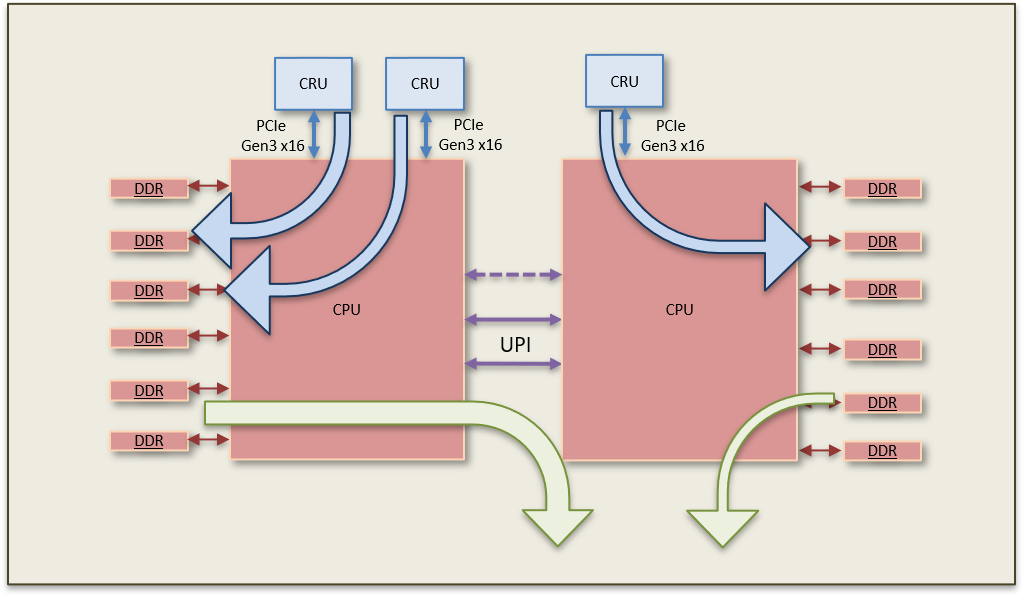
\includegraphics [width=100mm] {o2_flp/Readout_dataflows.png}
\caption{Simultaneous dataflows inside the FLP from the CRUs to the DDR memories and from the memory to the Infiniband network to the EPN farm.}
\label{fig_RO}
\end{figure}
%
 
%
%>>>>>>>>>>>>>>>>>>>>>>>>>>>>>>>>>>>>>>>>>>>>>>>>>>>>>>>>>> The data quality control 
%
\subsubsection{The data quality control}
The online execution of the calibration and the reconstruction and the replacement of the raw input data by reconstructed data, make the need for a reliable data Quality Control (QC) even more essential than usual. Its main motivations are to identify and help overcome problems during data taking and check that the data processing behaves as expected, thus ensuring good quality data for physics analyses.

The $O^2$  QC system \cite{ref_QC} is a distributed software as shown in Fig.\ref{fig_QC}.
    Data samples are selected following a pseudo-random sampling and configurable policies at key points in the data-flow and are dispatched to local (on the FLPs and the EPNs) or remote (on QC servers) QC tasks executing detector-specific algorithms. Their results are published as QC Objects, typically ROOT~\cite{ref_ROOT} histograms. The results of the QC tasks running in parallel on many nodes are assembled by the mergers.  
    Traditional or machine-learning-based checkers evaluate the quality of the objects and produce QC qualities. Finally the QC Objects and the Qualities are stored in the QC repository. This database uses the same technology as the Calibration and Condition DataBase of ALICE $O^2$. The Post-processing component encompasses asynchronous tasks such as correlation and trending of data derived from QC Objects and Qualities and triggered periodically, manually or on certain events (e.g. start of run or end of fill).
    QC and Quality Objects are accessible to shifters and experts through a web-based QC GUI.
%\end{itemize}
%
\begin{figure}[!h]
\centering
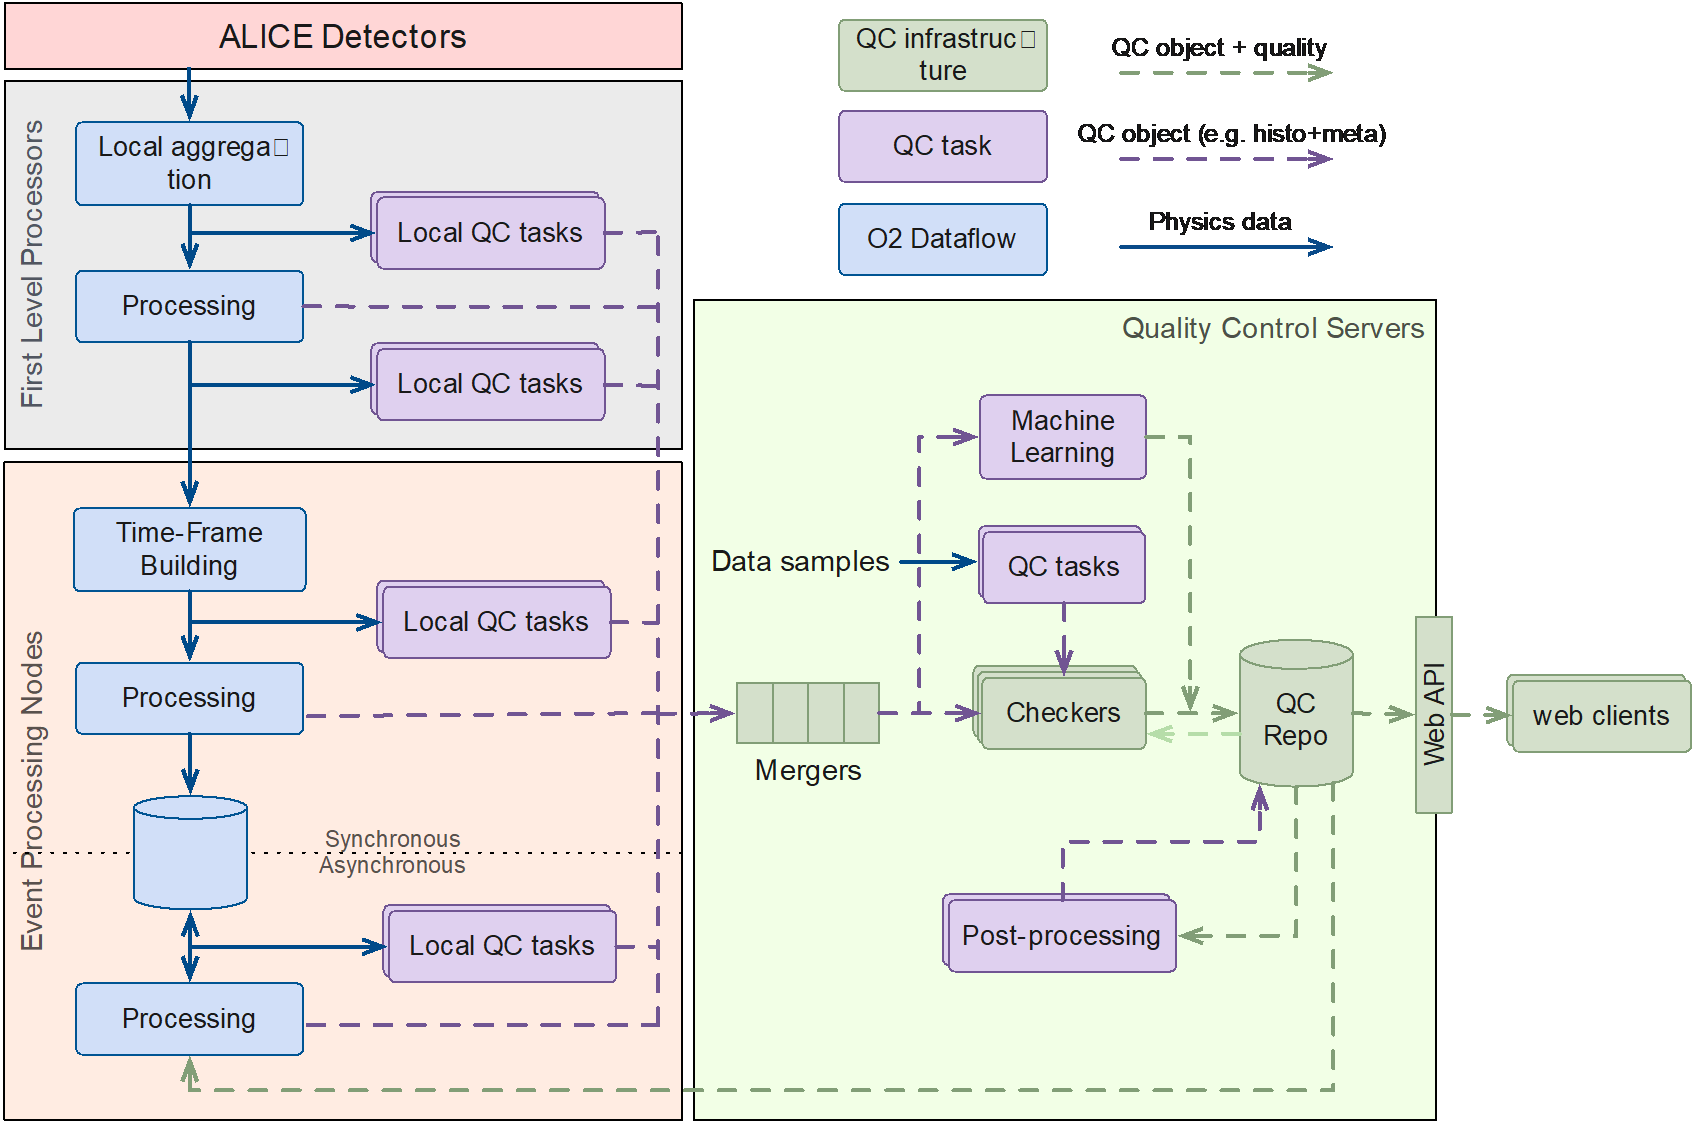
\includegraphics [width=100mm] {o2_flp/QC_Design.png}
\caption{$O^2$ Quality Control design.}
\label{fig_QC}
\end{figure}
%
%>>>>>>>>>>>>>>>>>>>>>>>>>>>>>>>>>>>>>>>>>>>>>>>>>>>>>>>>>> The services 
%
\subsubsection{The services}
%
%>>>>>>>>>>>>>>>>>>>>>>>>>>>>>>>>>>>>>>>>>>>>>>>>>>>>>>>>>> WebUI
\paragraph {Web User Interface framework}
Overview
The Web User Interface (Web UI) framework provides the core functionalities and building blocks to easily create rich web applications.
The server side features REST and WebSocket API, the authentication via CERN single sign-on and the authorisation using CERN e-groups.
The client-side features user interface Cascading Style Sheet building blocks, asynchronous data fetching (Ajax) and bi-directional socket (WebSockets).

%>>>>>>>>>>>>>>>>>>>>>>>>>>>>>>>>>>>>>>>>>>>>>>>>>>>>>>>>>> Control and configuration 
%
\paragraph{Control and configuration}
The ALICE Experiment Control System (AliECS) \cite{ref_aliecs} integrates the experiment control and configuration, the FLP farm control and a high-level control interface to the $O^2$/EPN cluster as shown in Fig~\ref{fig_aliecs}. It implements a distributed state machine to represent the aggregated state of the constituent $O^2$ processes of a data-driven workflow. Furthermore, it allows reconfiguration of running processes and simultaneous operation of multiple worflows, with easy reallocation of resources among workflows. Finally, it reacts promptly to inputs, handling events from the user, the LHC, the trigger system, the DCS, and the cluster itself with a high degree of autonomy. 

AliECS uses FairMQ, part of ALFA \cite{ref_alfa}, which is the common $O^2$ transport layer for physics data.   
Apache Mesos~\cite{ref_mesos} is a cluster resource management system, which facilitates the management of O2/FLP components, resources and tasks inside the O2/FLP facility, 
effectively enabling the developer to program against the datacenter (i.e., the O2/FLP facility at LHC Point 2) as if it was a single pool of resources. 

AliECS interfaces with Consul~\cite{ref_consul}, a key-value store which acts as the system’s configuration repository. The design also includes interfacing with information sources from the LHC, 
the trigger system, and the DCS. Once acquired by the AliECS core, configuration information is processed into an in-memory hierarchical key-value store, and from there it is
fed into a template system in order to generate task deployment and configuration structures.

Most components of AliECS are written in Go~\cite{ref_go}, a statically typed general purpose programming language in the tradition of C, which is particularly suitable for distributed system development because of its advanced synchronization and threading facilities.

\begin{figure}[!h]
\centering
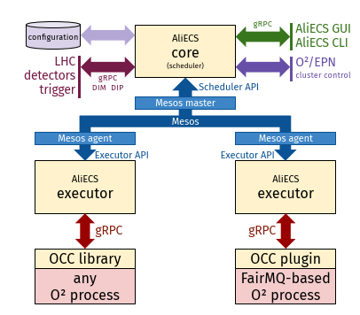
\includegraphics [width=100mm] {o2_flp/AliECS_Design.png}
\caption{AliECS design.}
\label{fig_aliecs}
\end{figure}

%
%>>>>>>>>>>>>>>>>>>>>>>>>>>>>>>>>>>>>>>>>>>>>>>>>>>>>>>>>>> Monitoring 
%
\paragraph{Monitoring}
The monitoring subsystem \cite{ref_monitor1, ref_monitor2} provides a complete overview of the overall system health, detects performance degradation and component failures by collecting, processing, storing and visualising values from hardware and software sensors and probes. As presented in Fig.~\ref{fig_monitoring}, metrics are sent to the system from both Telegraf \cite{ref_telegraf} (for system metrics) and the C++ monitoring library (via Telegraf, for application metrics). These metrics are processed in an Apache Kafka \cite{ref_Kafka} cluster and later written to InfluxDB \cite{ref_influxdb} time-series database for permanent storage.

InfluxDB time-series database supports downsampling which decreases the value resolution over time bringing down the total database size. It is planned to keep high resolution metrics for several days. After that time metrics will be downsampled in order to decrease the number of points and store them until the end of the calendar year. 

The system includes a data visualisation interface based on Grafana \cite{ref_grafana} and channels to email or mattermost for alarms and reporting.
\begin{figure}[!h]
\centering
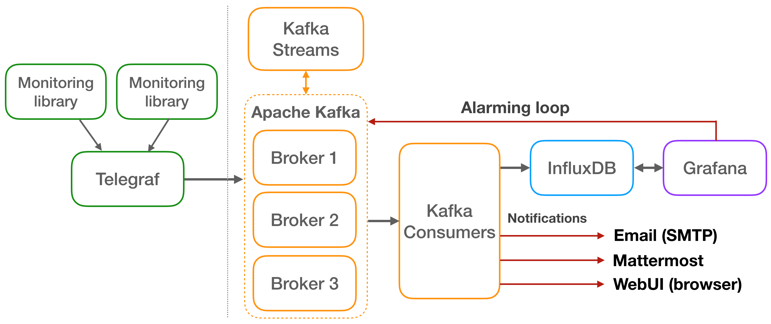
\includegraphics [width=100mm] {o2_flp/Monitoring_Design.png}
\caption{The $O^2$ computing system monitoring design.}
\label{fig_monitoring}
\end{figure}

%
%>>>>>>>>>>>>>>>>>>>>>>>>>>>>>>>>>>>>>>>>>>>>>>>>>>>>>>>>>> Logging 
%
\paragraph{Logging}
The logging system has been adapted from the ALICE Run 2 DAQ software \cite{ref_logging}. A new web-based user interface has been developed in addition to the existing GUIs.
%
%>>>>>>>>>>>>>>>>>>>>>>>>>>>>>>>>>>>>>>>>>>>>>>>>>>>>>>>>>> Bookkeeping 
%
\paragraph{Bookkeeping}
A new bookkeeping system called Jiskefet \cite{ref_bookkeeping} has been developed. It unifies two functionalities: gathering, storing and presenting metadata associated with the operations of the ALICE experiment and tracking the asynchronous processing of the physics data. The front end is based on the WebUI framework like the other applications and is adaptive to various clients such as tablets, mobile devices and other screens. The back end includes an OpenAPI specification based REST API and a relational database.


\subsection{EPN (Volker; 3p.)}
\subsection{Grid computing (Andreas; 3 p.)}
